\subsection{Multi-pool Load-balancing Performance}
\label{subsec:eval-multipool}
So far we have seen how our load-balancing policy performs within a single pool when all functions have the same priority level.
In this subsection, we evaluate the performance with \emph{multiple} priority levels and corresponding pools.
We are interested in the relative difference in performance between the pools, as well as how effectively we can provide service differentiation (by comparing to a single cluster).


\begin{comment}
Mainly centered around these evaluation questions:
\begin{enumerate}
\item What is the effect on the latency of high and low priority functions under various static cluster partitions?
\item What happens to cluster throughput?
\item Can cluster size be reduced? 
\item How does the dynamic partitioning affect performance under dynamic workloads? 
\end{enumerate}
\end{comment} 


\subsubsection{Two-pool performance}
For ease of exposition, we use two priority levels: high and low.
Functions are evenly assigned priority levels (i.e., half are high priority).
We use a cluster of size 8, with 4 servers in the high-priority pool. 
%For service differentiation, the high-priority pool is twice as large as the low-priority pool. 
%The cluster is evenly split between the high and low priority pools. 
%In the second case, we shrink (or deflate) the size of the lower priority pool, and thus the overall cluster size. This can potentially in


\begin{figure}
  \centering  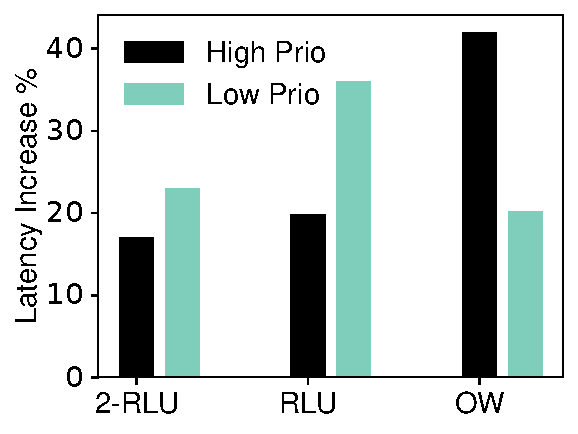
\includegraphics[width=0.7\textwidth]{chrlu/qos/Figures/fixed/qos1.pdf} %openload-latencies-cntnorm.png}
  \caption{Function prioritization improves latency for both high and low priority functions, and provides significant service differentiation and improvement over OpenWhisk.}
  \label{fig:qos:fixed-lat}
\end{figure}

Figure~\ref{fig:qos:fixed-lat} shows the increase in latency for both high and low priority functions, compared to their best-case warm start performance under no system load.
%We show latency increase, weighted by the relative frequency of the functions, to account for different function popularities. That is, we show sum of latency increase * function fraction in the workload.
The ``OW'' and ``RLU'' categories are the baseline performance in a single unpartitioned cluster without any function priorities.  
With 2 pools (2-RLU), we can see a that the latency of high-priority functions decreases compared to low-priority functions. 
By splitting the cluster in two, the locality \emph{increases}, and compared to the single-pool RLU, we see a decrease of 8\% in latency for high-priority and 10\% for low-priority functions. 
Compared to OpenWhisk, high-priority latency decreases by $5\times$, and low-priority latency \emph{increases} by 20\%, as OpenWhisk is not priority-aware.
Thus, $k$-RLU can provide significant service differentiation over OpenWhisk, improving performance for \emph{both} low and high priority functions compared to our single-pool RLU.

% Do we want to discuss throughput? Nah 

\subsubsection{Deflated lower-priority pool}

Service differentiation also allows us to \emph{reduce} the size of the low priority pool and thus the overall cluster size---improving utilization and efficiency.
We now evaluate function performance in such a differentiated setup.
Half the functions are low-priority, but the size of the low-priority pool is \emph{half} of that in the previous experiment.
That is, we shrink the initial cluster of 8 by 25\% to 6 servers, with 4 in the high-priority pool and only 2 in the low-priority pool.

\begin{figure}
  \centering 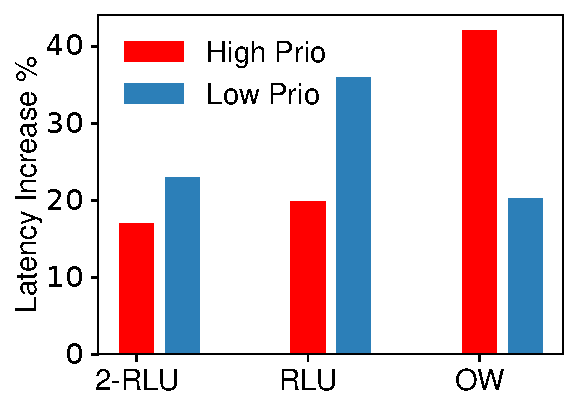
\includegraphics[width=0.7\textwidth]{chrlu/qos/Figures/fixed/qos2.pdf} %deflat/openload-latencies-cntnorm.png}
  \caption{Latencies on a 25\% smaller cluster. High-priority functions see a $2\times$ decrease vs. OpenWhisk.}
  \label{fig:qos:shrunk-lat}
\end{figure}

Figure~\ref{fig:qos:shrunk-lat} shows the latency in such a setup.
The single-pool RLU and OpenWhisk configurations are using the full original cluster size of 8 servers, while the 2-RLU has the 6 server configuration described above. 
Because of the reduction in total resources, the difference in performance between the 2-RLU and the single-pool methods like RLU and OpenWhisk is starker.
Compared to single-pool RLU, high-priority functions see a  10\% decrease in latency, and the low-priority functions see a decrease of 20\%.
Compared to OpenWhisk, we see a large 3x reduction in high-priority latency and an increase of 10\% in low-priority latency.
Thus, we can reduce the overall function latency by almost 2x \emph{even while reducing total cluster size by 25\%.}


A similar analysis of throughput is presented in Figure~\ref{fig:qos:shrunk-tput}. 
The 2-pool small cluster configuration achieves 12\% average higher throughput compared to OpenWhisk and 27\% compared to single-pool RLU.
Interestingly, RLU drops a larger number of functions owing to its strict load-bound, and thus achieves lower throughput. 


\begin{figure}
  \centering
  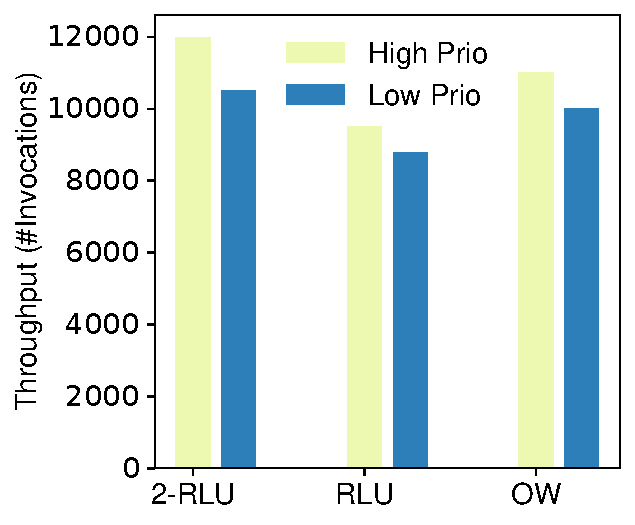
\includegraphics[width=0.7\textwidth]{chrlu/qos/Figures/fixed/tput2.pdf} %openload-throughputs.png}
  \caption[fixed-tput]{Throughput with deflatable cluster.}
  \label{fig:qos:shrunk-tput}
\end{figure}




%%% Local Variables:
%%% mode: latex
%%% TeX-master: "paper"
%%% End:
